\documentclass{beamer}
\usepackage[utf8]{inputenc}

\usetheme{Madrid}
\usecolortheme{default}
\usepackage{amsmath,amssymb,amsfonts,amsthm}
\usepackage{txfonts}
\usepackage{tkz-euclide}
\usepackage{listings}
\usepackage{adjustbox}
\usepackage{array}
\usepackage{tabularx}
\usepackage{gvv}
\usepackage{lmodern}
\usepackage{circuitikz}
\usepackage{tikz}
\usepackage{graphicx}
\usepackage{mathtools}

\setbeamertemplate{page number in head/foot}[totalframenumber]

\usepackage{tcolorbox}
\tcbuselibrary{minted,breakable,xparse,skins}



\definecolor{bg}{gray}{0.95}
\DeclareTCBListing{mintedbox}{O{}m!O{}}{%
  breakable=true,
  listing engine=minted,
  listing only,
  minted language=#2,
  minted style=default,
  minted options={%
    linenos,
    gobble=0,
    breaklines=true,
    breakafter=,,
    fontsize=\small,
    numbersep=8pt,
    #1},
  boxsep=0pt,
  left skip=0pt,
  right skip=0pt,
  left=25pt,
  right=0pt,
  top=3pt,
  bottom=3pt,
  arc=5pt,
  leftrule=0pt,
  rightrule=0pt,
  bottomrule=2pt,
  toprule=2pt,
  colback=bg,
  colframe=orange!70,
  enhanced,
  overlay={%
    \begin{tcbclipinterior}
    \fill[orange!20!white] (frame.south west) rectangle ([xshift=20pt]frame.north west);
    \end{tcbclipinterior}},
  #3,
}
\lstset{
    language=C,
    basicstyle=\ttfamily\small,
    keywordstyle=\color{blue},
    stringstyle=\color{orange},
    commentstyle=\color{green!60!black},
    numbers=left,
    numberstyle=\tiny\color{gray},
    breaklines=true,
    showstringspaces=false,
}
\title{5.2.48}
\date{27th September, 2025}
\author{Puni Aditya - EE25BTECH11046}

\begin{document}

\frame{\titlepage}
\begin{frame}{Question}
Solve the following system of linear equations.
\begin{align*}
    x+y+z&=1 \\
    2x+3y+2z&=2 \\
    ax+ay+2az&=4
\end{align*}
\end{frame}

\begin{frame}{Theoretical Solution}
\begin{align*}
    \myvec{1 & 1 & 1 \\ 2 & 3 & 2 \\ a & a & 2a}\myvec{x\\y\\z} &= \myvec{1\\2\\4}
\end{align*}
\begin{align}
    \myaugvec{3}{
        1 & 1 & 1 & 1 \\
        2 & 3 & 2 & 2 \\
        a & a & 2a & 4
    }
    \xleftrightarrow{\text{R}_3 \to \frac{1}{a}\text{R}_3, a \neq 0}
    \myaugvec{3}{
        1 & 1 & 1 & 1 \\
        2 & 3 & 2 & 2 \\
        1 & 1 & 2 & \frac{4}{a}
    }
\end{align}
\begin{align}
    \xleftrightarrow[\text{R}_3 \to \text{R}_3 - \text{R}_1]{\text{R}_2 \to \text{R}_2 - 2\text{R}_1}
    \myaugvec{3}{
        1 & 1 & 1 & 1 \\
        0 & 1 & 0 & 0 \\
        0 & 0 & 1 & \frac{4}{a} - 1
    }
    \xleftrightarrow{\text{R}_1 \to \text{R}_1 - \text{R}_2}
    \myaugvec{3}{
        1 & 0 & 1 & 1 \\
        0 & 1 & 0 & 0 \\
        0 & 0 & 1 & \frac{4}{a} - 1
    }
\end{align}
\end{frame}

\begin{frame}{Theoretical Solution}
\begin{align}
    \xleftrightarrow{\text{R}_1 \to \text{R}_1 - \text{R}_3}
    \myaugvec{3}{
        1 & 0 & 0 & 2 - \frac{4}{a} \\
        0 & 1 & 0 & 0 \\
        0 & 0 & 1 & \frac{4}{a} - 1
    }
\end{align}
\begin{align}
    \myvec{x\\y\\z} &= \myvec{2 - \frac{4}{a} \\ 0 \\ \frac{4}{a} - 1},\text{ }a \neq 0 \label{eq:65}
\end{align}
For $a=0$, the third equation becomes $0=4$, which is inconsistent. Therefore, no solution exists for $a=0$.
\end{frame}

\begin{frame}{Example}
Let
\begin{align*}
    a = 2
\end{align*}
\begin{align*}
    x+y+z&=1 \\
    2x+3y+2z&=2 \\
    2x+2y+4z&=4
\end{align*}
\begin{align*}
    \myvec{1 & 1 & 1 \\ 2 & 3 & 2 \\ 2 & 2 & 4}\myvec{x\\y\\z} &= \myvec{1\\2\\4}
\end{align*}
Using \eqref{eq:65},
\begin{align}
    \myvec{x\\y\\z} &= \myvec{0 \\ 0 \\ 1}
\end{align}
\end{frame}

\begin{frame}{Plot}
    \begin{figure}
        \centering
        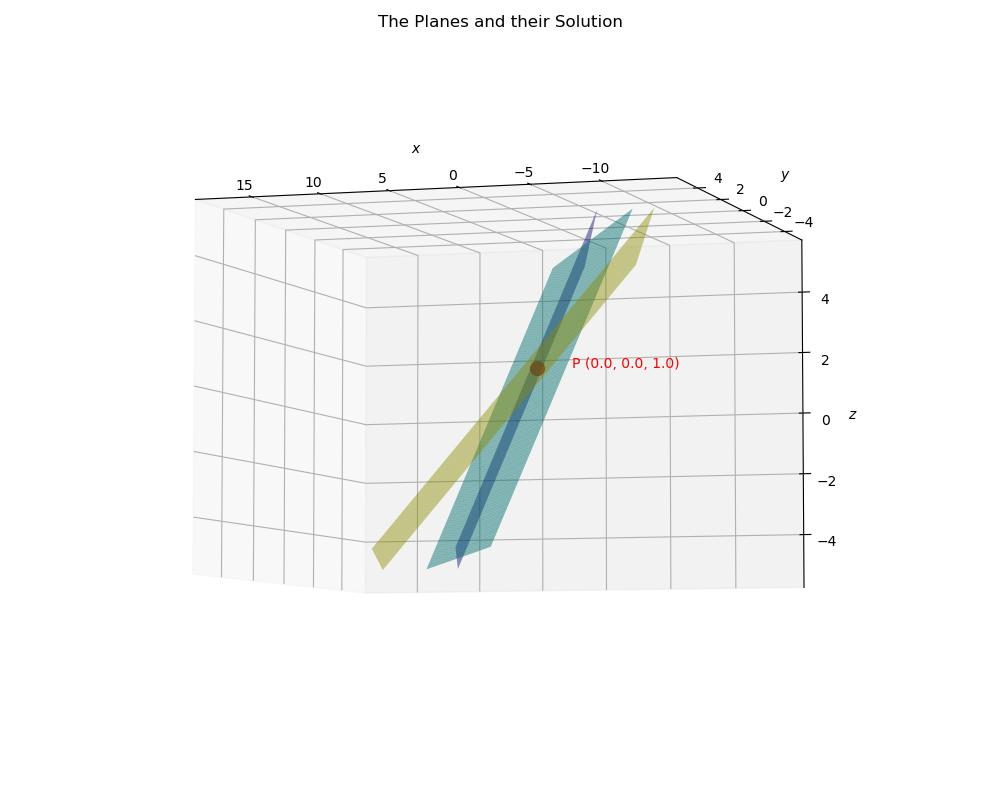
\includegraphics[width=0.5\columnwidth]{../figs/plot_c.jpg}
        \caption{Plot}
        \label{fig:fig}
    \end{figure}
\end{frame}

\end{document}
